 \documentclass[12pt]{article}
%% note that some of the references from the answers were changed by hand
%% search for Section and Figure
  \usepackage{wrapfig}
 \input{mystyle.sty}
    \usepackage{proof}
    \usepackage{url}
    \usepackage{fitch}
    \usepackage[all]{xy}  
      \usepackage{enumitem}
%\thispagestyle{empty}
\usepackage{tikz}
\usetikzlibrary{arrows,shapes,snakes,automata,backgrounds,petri,trees}
\usepackage{pifont}
\usepackage{pxfonts} 
\oddsidemargin 0pt
\evensidemargin 0 pt
\topmargin -.3in
\headsep 20pt
\footskip 20pt
\textheight 8.5in
\textwidth 6.25in
%\newcommand{\cal}[1]{\mathcal{#1}}
% Alter some LaTeX defaults for better treatment of figures:
    % See p.105 of "TeX Unbound" for suggested values.
    % See pp. 199-200 of Lamport's "LaTeX" book for details.
    %   General parameters, for ALL pages:
%    \renewcommand{\truefraction}{0.9}	% max fraction of floats at top
%    \renewcommand{\falsetomfraction}{0.8}	% max fraction of floats at bottom
    %   Para meters for TEXT pages (not float pages):
    \setcounter{topnumber}{2}
    \setcounter{bottomnumber}{2}
    \setcounter{totalnumber}{4}     % 2 may work better
    \setcounter{dbltopnumber}{2}    % for 2-column pages
    \renewcommand{\dbltopfraction}{0.9}	% fit big float above 2-col. text
    \renewcommand{\textfraction}{0.07}	% allow minimal text w. figs
    %   Parameters for FLOAT pages (not text pages):
    \renewcommand{\floatpagefraction}{0.7}	% require fuller float pages
	% N.B.: floatpagefraction MUST be less than topfraction !!
    \renewcommand{\dblfloatpagefraction}{0.7}	% require fuller float pages


\renewcommand\thesubsection{\arabic{subsection}}

 \begin{document}


\begin{center}
{
\Large  Modal Logic, Winter 2019   \\
   Homework 4 
\\
due Tuesday, February 5 \\
} 
\end{center}


\subsection{Review of modal semantics on graphs}\label{graph}
Recall the following graph from Homework 3.
 $$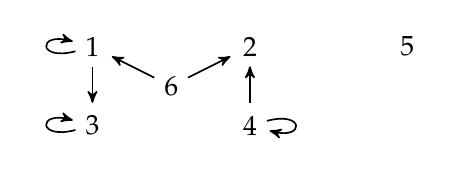
\begin{tikzpicture}[<->,>=stealth',shorten >=1pt,auto,node distance=5cm,semithick]
\node (a) at (-1,0) {$3$}
          edge [loop left] node {} (a)
   ;
\node (b) at (1,0) {$4$}
       edge [loop right]   node     [swap]   {}            (b)       
;
\node (c) at (-1,1) {$1$}
               edge [loop left] node {} (c)
                      % edge [pre] node {} (a)
         edge [post] node {} (a)
                ;
\node (d) at (1,1) {$2$}
         %     edge [loop right] node {} (d)
                     edge [<-] node {} (b)                     
; 
\node (e) at (3,1) {$5$};
\node (f) at (0,.5) {$6$}
edge [->] node {} (c)  
edge [->] node {} (d)  
;
\end{tikzpicture}
$$
We saw on that homework that the following partition $\Pi$ had the property that $\refine(\GG,\Pi)=\Pi$:
$\set{\set{1,3},\set{4},\set{6},\set{2,5}}$.
\begin{enumerate}
\item Find a modal logic sentence $\phi_1$ such that $1\models \phi$, $4\not\models\phi$, $6\not\models\phi$, and $2\not\models\phi$.
\item Does $3\models\phi_1$ as well?
\item Find a modal logic sentence $\phi_4$ such that $1\not\models \phi$, $4\models\phi$, $6\not\models\phi$, and $2\not\models\phi$.
\item Find a modal logic sentence $\phi_6$ such that $1\not\models \phi$, $4\not\models\phi$, $6\models\phi$, and $2\not\models\phi$.

\item Find a modal logic sentence $\phi_2$ such that $1\not\models \phi$, $4\not\models\phi$, $6\not\models\phi$, and $2\models\phi$.
\item Does $5\models\phi_2$ as well?
\end{enumerate}
You can use the inductive method from Tuesday's class, or you could just guess the answer.
You don't have to justify your assertions, but I trust that you \emph{could} write out the full justifications if you needed to.



\subsection{Facts about modal semantics on graphs}
\begin{enumerate}
\item Let $\GG = (G,\to)$ be a Euclidean graph.
Show that for all $g\in G$ $g\models \poss p\iif \necc \poss p$.
\item Is the following true:  for every modal sentence $\phi$, the sentence 
$\poss \phi \iif \necc \poss \phi$
is true at every point in every Euclidean graph?\label{whatwould}
\item 
 Let $\GG = (G,\to)$ be a graph which is a partial function.
Show that for all $g\in G$ $g\models \poss p\iif \necc  p$.
\item What would the analog of part (\ref{whatwould}) be for partial function graphs?



\end{enumerate}


\subsection{A fact about fixed points of monotone functions on posets}

Recall that a \emph{partially-ordered set} (also called a \emph{poset}) is a preorder $(P,\leq)$ which
is antisymmetric.

Let $(P,\leq)$ be a poset, and suppose that $P$ has a least element, $\bot$.
(This is read ``bottom.'') Let $f:P\to P$ monotone,
and let $p^*$ be a fixed point of $f$.   Show that for all $n$, $f^n(\bot) \leq p^*$.

Here is what this means in more detail.
We assume that $f$ has the following property: if $p\leq q$, then $f(p) \leq f(q)$.
We define elements $f^n(\bot)$ of $P$ by the following recursion:
$f^0(\bot) = \bot$, and $f^{n+1}(\bot) = f(f^n(\bot)$.
Finally, we fix an element $p^*$ such that $f(p^*)= p^*$.
We want to prove that for all $n$ $f^n(\bot) \leq p^*$.
\label{part-monotone}

\subsection{Another fact about fixed points of monotone functions on posets, this time finite posets}
\label{anotherfact}
As in problem~\ref{part-monotone}, let 
 $(P,\leq)$ be a poset, and suppose that $P$ has a least element, $\bot$.
Let $f:P\to P$ monotone,

\begin{enumerate}
\item If $P$ is \emph{finite}, then show that there is some $n$ such that $f^n(\bot) = f^{n+1}(\bot)$.

[Use the following fact:  If $A$ is any finite set, and if $a_0, a_1, a_2, \ldots, a_n, \ldots$ is an infinite
sequence from $A$, then there must be $i < j$ such that $a_i = a_j$.]
\label{existsfp}
\item Given an example to show that we need $P$ to be finite in order to have the result in   part (\ref{existsfp}).
\item Use part (\ref{existsfp}) and results from Homework 3 to show that for every \emph{finite} graph $\GG$, there is a partition 
$\Pi$ of the nodes of the graph such that $\Pi = \refine(\GG,\Pi)$.  [Hint: 
  Recall from Homework 3, problem 3 that the set $P$ of partitions of $G$ is a poset, where $\leq$ is the refinement 
order.   What is the $\bot$ of this order?   And what monotone function on $P$ should we think about?]

\end{enumerate}
\label{existsfpartition}


\subsection{Modal sentences and partitions}\label{fixedpointimpliesequivalence}
Let $\GG$ be a graph.   Recall that we interpret the modal language with $\true$, $\false$, $\nott$, $\andd$, $\orr$, $\iif$, $\iiff$, $\necc$, and $\poss$ on $\GG$.
Let $\Pi$ be a partition  of the nodes of $\GG$ such that 
$\Pi = \refine(\GG,\Pi)$.   In this problem, we are going to prove that
for all modal sentences $\phi$ the following holds:
\[\begin{array}{l}
\underline{\mbox{for all $g, h\in G$}},\\
\underline{\mbox{if $g$ and $h$ belong to the same cell of $\Pi$,
then $g\models\phi$ if and only if $h\models\phi$.}}
\end{array}
\]
\begin{enumerate}
\item Write out the underlined statement with $\phi$ being $\true$, and say why the statement you wrote is true.
(The same holds for $\false$, but we'll skip this.)
\item  This next part is the induction step for $\andd$.
Take   sentences $\phi$ and $\psi$, and  assume the underlined statement for $\phi$ and also the underlined statement for $\psi$.
Write out these assumptions.   Then write your goal: the underlined statement for the sentence $\phi\andd\psi$.
Prove this statement.   The argument should be easy.

We are going to skip the induction steps for $\nott$, $\orr$, $\iif$, and $\iiff$, since they are basically the same as the one for $\andd$.
\item This next part is the induction step for $\poss$.
Take a  sentence  $\phi$,   assume the underlined statement for $\phi$, and prove it for $\poss\phi$.
You will definitely need to use the assumption that $\Pi = \refine(\GG,\Pi)$ in this part, so be sure to indicate where exactly this assumption was used.
\item This next part is the induction step for $\necc$.
Take a  sentence  $\phi$,   assume the underlined statement for $\phi$, and prove it for $\necc\phi$.
You will definitely again need to use the assumption that $\Pi = \refine(\GG,\Pi)$ in this part, so be sure to indicate where exactly this assumption was used.
[The step  for $\necc$ is quite close to the step for $\poss$, but you should start with the one for $\poss$ because it is a little easier.]
\end{enumerate}

\subsection{Putting it all together}
Let $\GG$ be a finite graph.  
\begin{enumerate}
\item Let $\equiv$ be the following  relation on the nodes of $G$:
\[ g \equiv h \quadiff \mbox{$g$ and $h$ satisfy the same modal sentences} \]
Check that $\equiv$ is an equivalence relation.  [This should be easy.]
\item Let $\Pi_{1}$ be the partition associated to $\equiv$.   
In the special example of the graph $\GG$ in Exercise~\ref{graph}, what  exactly are the cells of $\Pi_1$, and why?
\item
  Recall from 
problem~\ref{existsfpartition} that 
for every finite graph $\GG$, 
there is some number $n$ so that  $f^n(\bot)$ which is a fixed point of refinement:
$\refine(f^n(\bot)) = f^n(\bot)$.  (That is, for some particular $n$, this holds.)   Let $\Pi_2$ be such a partition.
So, for some numberr $N$, $\Pi_2 =  f^N(\bot)$. 
 Prove that for all finite graphs $\GG$, $\Pi_1 = \Pi_2$.
 [The point here is to quote other results: so look at this homework and the previous one, and also what we did in class.]
 

 
\end{enumerate} 
\end{document}

